\documentclass[a4paper]{book}
\usepackage{makeidx}
\usepackage{graphicx}
\usepackage{multicol}
\usepackage{float}
\usepackage{listings}
\usepackage{color}
\usepackage{textcomp}
\usepackage{alltt}
\usepackage{times}
\usepackage{ifpdf}
\ifpdf
\usepackage[pdftex,
            pagebackref=true,
            colorlinks=true,
            linkcolor=blue,
            unicode
           ]{hyperref}
\else
\usepackage[ps2pdf,
            pagebackref=true,
            colorlinks=true,
            linkcolor=blue,
            unicode
           ]{hyperref}
\usepackage{pspicture}
\fi
\usepackage[utf8]{inputenc}
\usepackage[french]{babel}

\usepackage{doxygen}
\lstset{language=C++,inputencoding=utf8,basicstyle=\footnotesize,breaklines=true,breakatwhitespace=true,tabsize=8,numbers=left }
\makeindex
\setcounter{tocdepth}{3}
\renewcommand{\footrulewidth}{0.4pt}
\begin{document}
\hypersetup{pageanchor=false}
\begin{titlepage}
\vspace*{7cm}
\begin{center}
{\Large Editeur-\/Web }\\
\vspace*{1cm}
{\large Généré par Doxygen 1.7.1}\\
\vspace*{0.5cm}
{\small Wed Apr 17 2013 21:54:37}\\
\end{center}
\end{titlepage}
\clearemptydoublepage
\pagenumbering{roman}
\tableofcontents
\clearemptydoublepage
\pagenumbering{arabic}
\hypersetup{pageanchor=true}
\chapter{Index des espaces de nommage}
\section{Liste des espaces de nommage}
Liste de tous les espaces de nommage documentés avec une brève description:\begin{DoxyCompactList}
\item\contentsline{section}{\hyperlink{namespaceUi}{Ui} }{\pageref{namespaceUi}}{}
\end{DoxyCompactList}

\chapter{Index des classes}
\section{Class Hierarchy}
This inheritance list is sorted roughly, but not completely, alphabetically\-:\begin{DoxyCompactList}
\item \contentsline{section}{Buffer}{\pageref{class_buffer}}{}
\item \contentsline{section}{Dom}{\pageref{class_dom}}{}
\item \contentsline{section}{Facteur}{\pageref{class_facteur}}{}
\item \contentsline{section}{Ligne}{\pageref{class_ligne}}{}
\item \contentsline{section}{Noeud}{\pageref{class_noeud}}{}
\item \contentsline{section}{noeudtexte}{\pageref{classnoeudtexte}}{}
\item \contentsline{section}{nom}{\pageref{classnom}}{}
\item Q\-Main\-Window\begin{DoxyCompactList}
\item \contentsline{section}{Le\-Edit}{\pageref{class_le_edit}}{}
\end{DoxyCompactList}
\end{DoxyCompactList}

\chapter{Index des classes}
\section{\-Liste des classes}
\-Liste des classes, structures, unions et interfaces avec une brève description \-:\begin{DoxyCompactList}
\item\contentsline{section}{\hyperlink{classBuffer}{\-Buffer} }{\pageref{classBuffer}}{}
\item\contentsline{section}{\hyperlink{classfacteur}{facteur} }{\pageref{classfacteur}}{}
\item\contentsline{section}{\hyperlink{classLeEdit}{\-Le\-Edit} }{\pageref{classLeEdit}}{}
\item\contentsline{section}{\hyperlink{classLigne}{\-Ligne} }{\pageref{classLigne}}{}
\end{DoxyCompactList}

\chapter{Index des fichiers}
\section{File List}
Here is a list of all documented files with brief descriptions\-:\begin{DoxyCompactList}
\item\contentsline{section}{\hyperlink{buffer_8cc}{buffer.\-cc} }{\pageref{buffer_8cc}}{}
\item\contentsline{section}{{\bfseries buffer.\-h} }{\pageref{buffer_8h}}{}
\item\contentsline{section}{{\bfseries dom.\-h} }{\pageref{dom_8h}}{}
\item\contentsline{section}{\hyperlink{facteur_8cc}{facteur.\-cc} }{\pageref{facteur_8cc}}{}
\item\contentsline{section}{\hyperlink{facteur_8h}{facteur.\-h} }{\pageref{facteur_8h}}{}
\item\contentsline{section}{{\bfseries leedit.\-h} }{\pageref{leedit_8h}}{}
\item\contentsline{section}{\hyperlink{ligne_8cc}{ligne.\-cc} }{\pageref{ligne_8cc}}{}
\item\contentsline{section}{{\bfseries ligne.\-h} }{\pageref{ligne_8h}}{}
\item\contentsline{section}{{\bfseries noeud.\-h} }{\pageref{noeud_8h}}{}
\item\contentsline{section}{{\bfseries noeudtexte.\-h} }{\pageref{noeudtexte_8h}}{}
\end{DoxyCompactList}

\chapter{Documentation des espaces de nommage}
\hypertarget{namespaceUi}{
\section{Référence de l'espace de nommage Ui}
\label{namespaceUi}\index{Ui@{Ui}}
}


\subsection{Description détaillée}
espace de nommage regroupant les outils composants de l'interface graphique 
\chapter{Documentation des classes}
\hypertarget{classBuffer}{\section{\-Référence de la classe \-Buffer}
\label{classBuffer}\index{\-Buffer@{\-Buffer}}
}
\subsection*{\-Fonctions membres publiques}
\begin{DoxyCompactItemize}
\item 
\hypertarget{classBuffer_a968f9c9b50fe02f7d76de200f78507b0}{{\bfseries \-Buffer} (char chemin\-Fichier\mbox{[}$\,$\mbox{]})}\label{classBuffer_a968f9c9b50fe02f7d76de200f78507b0}

\item 
\hypertarget{classBuffer_aaa71afa6da49b147a7060900288e67d3}{void {\bfseries ajouter\-Ligne} (\hyperlink{classLigne}{\-Ligne} l, int position)}\label{classBuffer_aaa71afa6da49b147a7060900288e67d3}

\item 
\hypertarget{classBuffer_ae3c4df1d65179d391de936a324c48871}{\-D\-O\-M {\bfseries get\-Dom} () const }\label{classBuffer_ae3c4df1d65179d391de936a324c48871}

\item 
\hypertarget{classBuffer_ab0d9e2abf2c5a8390d567407cd1cf556}{void {\bfseries set\-Dom} (const \-D\-O\-M \&)}\label{classBuffer_ab0d9e2abf2c5a8390d567407cd1cf556}

\item 
\hypertarget{classBuffer_af7f5a6f316e5659e462874998c87921d}{list$<$ \hyperlink{classLigne}{\-Ligne} $>$ {\bfseries get\-Lignes} () const }\label{classBuffer_af7f5a6f316e5659e462874998c87921d}

\item 
\hypertarget{classBuffer_a8d4cb25f19d9782d663d73ca460e1e37}{void {\bfseries set\-Lignes} (const list$<$ \hyperlink{classLigne}{\-Ligne} $>$ \&)}\label{classBuffer_a8d4cb25f19d9782d663d73ca460e1e37}

\item 
\hypertarget{classBuffer_a122fe744cef772a83c6228195474171d}{void {\bfseries set\-Lignes} (char chemin\-Fichier\mbox{[}$\,$\mbox{]})}\label{classBuffer_a122fe744cef772a83c6228195474171d}

\item 
\hypertarget{classBuffer_a89c9eac6ff51f0e9b2e8eaddd1c56bd0}{void {\bfseries affiche} (ostream \&) const }\label{classBuffer_a89c9eac6ff51f0e9b2e8eaddd1c56bd0}

\item 
\hypertarget{classBuffer_a9dddb1a46c258c5db1ed04a101e0a5cd}{void {\bfseries saisie} (istream \&)}\label{classBuffer_a9dddb1a46c258c5db1ed04a101e0a5cd}

\item 
\hypertarget{classBuffer_aa9f3fc3d9114811eba3029072eaf10fa}{void {\bfseries sauv\-Temp} ()}\label{classBuffer_aa9f3fc3d9114811eba3029072eaf10fa}

\item 
\hypertarget{classBuffer_aeddaa4c55df7da9daa8541157fc4f096}{void {\bfseries maj\-D\-O\-M} ()}\label{classBuffer_aeddaa4c55df7da9daa8541157fc4f096}

\end{DoxyCompactItemize}


\-La documentation de cette classe a été générée à partir des fichiers suivants \-:\begin{DoxyCompactItemize}
\item 
buffer.\-h\item 
buffer.\-cc\end{DoxyCompactItemize}

\hypertarget{classDom}{
\section{Référence de la classe Dom}
\label{classDom}\index{Dom@{Dom}}
}
\subsection*{Fonctions membres publiques}
\begin{DoxyCompactItemize}
\item 
\hypertarget{classDom_a3760e9581e6764d429fc68d070546f3f}{
{\bfseries Dom} (\hyperlink{classNoeud}{Noeud} \&)}
\label{classDom_a3760e9581e6764d429fc68d070546f3f}

\item 
\hypertarget{classDom_ae02da1237c5c884af49ea992417cfdcd}{
{\bfseries Dom} (list$<$ \hyperlink{classLigne}{Ligne} $>$)}
\label{classDom_ae02da1237c5c884af49ea992417cfdcd}

\item 
\hypertarget{classDom_ae640a720c988454576287a5b6c083a6a}{
virtual bool {\bfseries ajoutNoeud} (const \hyperlink{classNoeud}{Noeud} \&, const \hyperlink{classNoeud}{Noeud} \&)}
\label{classDom_ae640a720c988454576287a5b6c083a6a}

\item 
\hypertarget{classDom_ab700f17d298e9d403d1189e6cbd2e21e}{
virtual bool {\bfseries noeudPresent} (const \hyperlink{classNoeud}{Noeud} \&)}
\label{classDom_ab700f17d298e9d403d1189e6cbd2e21e}

\item 
\hypertarget{classDom_abae2486b2f93b2c45e3ff830219488b2}{
virtual istream \& {\bfseries saisie} (istream \&)}
\label{classDom_abae2486b2f93b2c45e3ff830219488b2}

\item 
\hypertarget{classDom_a692547ba6010fd70040e8b4ab2805349}{
virtual ostream \& {\bfseries affiche} (ostream \&) const }
\label{classDom_a692547ba6010fd70040e8b4ab2805349}

\item 
\hypertarget{classDom_ab7755b82fa26674d7d31833a0a38887b}{
virtual int {\bfseries nbNoeud} () const }
\label{classDom_ab7755b82fa26674d7d31833a0a38887b}

\item 
\hypertarget{classDom_a50701606026b355374e210ca659d9738}{
virtual int {\bfseries retournerTabLigne} (\hyperlink{classNoeud}{Noeud} \&)}
\label{classDom_a50701606026b355374e210ca659d9738}

\item 
\hypertarget{classDom_a227c734caf6f1d36a7cf5b21306b240b}{
virtual \hyperlink{classNoeud}{Noeud} {\bfseries retournerPtrNode} (\hyperlink{classLigne}{Ligne} \&)}
\label{classDom_a227c734caf6f1d36a7cf5b21306b240b}

\end{DoxyCompactItemize}


La documentation de cette classe a été générée à partir des fichiers suivants :\begin{DoxyCompactItemize}
\item 
dom.h\item 
dom.cc\end{DoxyCompactItemize}

\hypertarget{classDOMText}{
\section{Référence de la classe DOMText}
\label{classDOMText}\index{DOMText@{DOMText}}
}
Graphe d'héritage de DOMText:\begin{figure}[H]
\begin{center}
\leavevmode
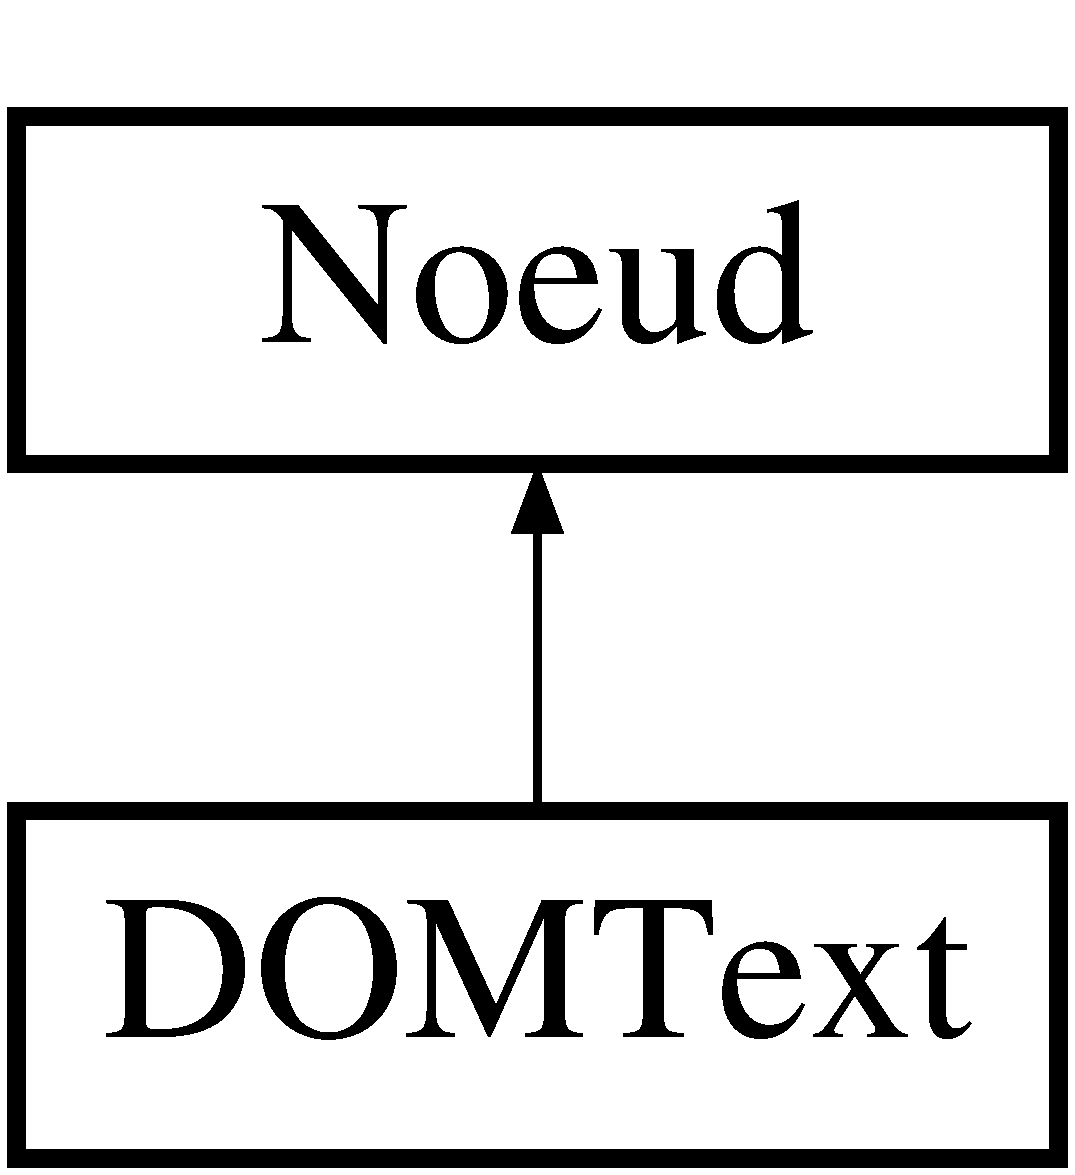
\includegraphics[height=2.000000cm]{classDOMText}
\end{center}
\end{figure}
\subsection*{Fonctions membres publiques}
\begin{DoxyCompactItemize}
\item 
\hypertarget{classDOMText_a92469df02e0f2cd52726e3194e371fc7}{
{\bfseries noeudtexte} ()}
\label{classDOMText_a92469df02e0f2cd52726e3194e371fc7}

\item 
\hypertarget{classDOMText_ae256521159a51eed8ace13933af3aac5}{
void {\bfseries setText} (string)}
\label{classDOMText_ae256521159a51eed8ace13933af3aac5}

\end{DoxyCompactItemize}


La documentation de cette classe a été générée à partir du fichier suivant :\begin{DoxyCompactItemize}
\item 
noeudtexte.h\end{DoxyCompactItemize}

\hypertarget{classFacteur}{
\section{Référence de la classe Facteur}
\label{classFacteur}\index{Facteur@{Facteur}}
}
\subsection*{Fonctions membres publiques}
\begin{DoxyCompactItemize}
\item 
\hypertarget{classFacteur_a989e3e6f53f97d5adfd2e7e3fc1f4cf1}{
\hyperlink{classFacteur_a989e3e6f53f97d5adfd2e7e3fc1f4cf1}{Facteur} ()}
\label{classFacteur_a989e3e6f53f97d5adfd2e7e3fc1f4cf1}

\begin{DoxyCompactList}\small\item\em Constructeur par défaut. \item\end{DoxyCompactList}\item 
\hyperlink{classFacteur_af0d4423b4ebe026d9dbe8ef06eb23d9f}{Facteur} (char $\ast$text)
\begin{DoxyCompactList}\small\item\em Constructeur de facteur. \item\end{DoxyCompactList}\item 
\hypertarget{classFacteur_a71486fcb174b3a49520bf1e60fbf8e69}{
\hyperlink{classFacteur_a71486fcb174b3a49520bf1e60fbf8e69}{$\sim$Facteur} ()}
\label{classFacteur_a71486fcb174b3a49520bf1e60fbf8e69}

\begin{DoxyCompactList}\small\item\em Destructeur de facteur. \item\end{DoxyCompactList}\item 
void \hyperlink{classFacteur_aa83b5bd6563b1f2cab21dddd90fc6666}{setTexte} (char $\ast$text)
\begin{DoxyCompactList}\small\item\em Definir le texte. \item\end{DoxyCompactList}\item 
char $\ast$ \hyperlink{classFacteur_afb04776df3a588d1d52a227854ab37a1}{getTexte} ()
\begin{DoxyCompactList}\small\item\em Retourne le texte du facteur. \item\end{DoxyCompactList}\item 
char $\ast$ \hyperlink{classFacteur_a887bb35c1fdff90040c91716abd15d62}{getTexteFormate} ()
\begin{DoxyCompactList}\small\item\em Retourne le texte du facteur formaté avec la couleur. \item\end{DoxyCompactList}\item 
void \hyperlink{classFacteur_ad17a1b26444aee5f6a474296c47c134a}{setCouleur} (char $\ast$color)
\begin{DoxyCompactList}\small\item\em Definir la couleur. \item\end{DoxyCompactList}\item 
\hypertarget{classFacteur_a16f36a57adf914658c50fbd527f2e2b8}{
void \hyperlink{classFacteur_a16f36a57adf914658c50fbd527f2e2b8}{formate} ()}
\label{classFacteur_a16f36a57adf914658c50fbd527f2e2b8}

\begin{DoxyCompactList}\small\item\em Formate puis stock le texte. \item\end{DoxyCompactList}\end{DoxyCompactItemize}


\subsection{Description détaillée}
surcharge de l'operateur $<$$<$ 

\subsection{Documentation des constructeurs et destructeur}
\hypertarget{classFacteur_af0d4423b4ebe026d9dbe8ef06eb23d9f}{
\index{Facteur@{Facteur}!Facteur@{Facteur}}
\index{Facteur@{Facteur}!Facteur@{Facteur}}
\subsubsection[{Facteur}]{\setlength{\rightskip}{0pt plus 5cm}Facteur::Facteur (
\begin{DoxyParamCaption}
\item[{char $\ast$}]{ text}
\end{DoxyParamCaption}
)}}
\label{classFacteur_af0d4423b4ebe026d9dbe8ef06eb23d9f}


Constructeur de facteur. 


\begin{DoxyParams}{Paramètres}
\item[{\em text}]texte du facteur \end{DoxyParams}


\subsection{Documentation des fonctions membres}
\hypertarget{classFacteur_afb04776df3a588d1d52a227854ab37a1}{
\index{Facteur@{Facteur}!getTexte@{getTexte}}
\index{getTexte@{getTexte}!Facteur@{Facteur}}
\subsubsection[{getTexte}]{\setlength{\rightskip}{0pt plus 5cm}char $\ast$ Facteur::getTexte (
\begin{DoxyParamCaption}
{}
\end{DoxyParamCaption}
)}}
\label{classFacteur_afb04776df3a588d1d52a227854ab37a1}


Retourne le texte du facteur. 

\begin{DoxyReturn}{Renvoie}
retourne le texte du facteur 
\end{DoxyReturn}
\hypertarget{classFacteur_a887bb35c1fdff90040c91716abd15d62}{
\index{Facteur@{Facteur}!getTexteFormate@{getTexteFormate}}
\index{getTexteFormate@{getTexteFormate}!Facteur@{Facteur}}
\subsubsection[{getTexteFormate}]{\setlength{\rightskip}{0pt plus 5cm}char $\ast$ Facteur::getTexteFormate (
\begin{DoxyParamCaption}
{}
\end{DoxyParamCaption}
)}}
\label{classFacteur_a887bb35c1fdff90040c91716abd15d62}


Retourne le texte du facteur formaté avec la couleur. 

\begin{DoxyReturn}{Renvoie}
retourne le texte du facteur formate 
\end{DoxyReturn}
\hypertarget{classFacteur_ad17a1b26444aee5f6a474296c47c134a}{
\index{Facteur@{Facteur}!setCouleur@{setCouleur}}
\index{setCouleur@{setCouleur}!Facteur@{Facteur}}
\subsubsection[{setCouleur}]{\setlength{\rightskip}{0pt plus 5cm}void Facteur::setCouleur (
\begin{DoxyParamCaption}
\item[{char $\ast$}]{ color}
\end{DoxyParamCaption}
)}}
\label{classFacteur_ad17a1b26444aee5f6a474296c47c134a}


Definir la couleur. 


\begin{DoxyParams}{Paramètres}
\item[{\em color}]couleur du facteur \end{DoxyParams}
\hypertarget{classFacteur_aa83b5bd6563b1f2cab21dddd90fc6666}{
\index{Facteur@{Facteur}!setTexte@{setTexte}}
\index{setTexte@{setTexte}!Facteur@{Facteur}}
\subsubsection[{setTexte}]{\setlength{\rightskip}{0pt plus 5cm}void Facteur::setTexte (
\begin{DoxyParamCaption}
\item[{char $\ast$}]{ text}
\end{DoxyParamCaption}
)}}
\label{classFacteur_aa83b5bd6563b1f2cab21dddd90fc6666}


Definir le texte. 


\begin{DoxyParams}{Paramètres}
\item[{\em text}]texte du facteur \end{DoxyParams}


La documentation de cette classe a été générée à partir des fichiers suivants :\begin{DoxyCompactItemize}
\item 
\hyperlink{facteur_8h}{facteur.h}\item 
\hyperlink{facteur_8cc}{facteur.cc}\end{DoxyCompactItemize}

\hypertarget{classLeEdit}{
\section{Référence de la classe LeEdit}
\label{classLeEdit}\index{LeEdit@{LeEdit}}
}


Classe gérant l'interface graphique.  




{\ttfamily \#include $<$leedit.h$>$}

\subsection*{Connecteurs publics}
\begin{DoxyCompactItemize}
\item 
void \hyperlink{classLeEdit_a093399eb39cfb60f825ecbc6ab5ae096}{affichageDOM} (bool visible)
\begin{DoxyCompactList}\small\item\em affichageDOM Affiche ou cache la fenêtre DOM \item\end{DoxyCompactList}\item 
void \hyperlink{classLeEdit_ad4ae5c310f20d825dc582f8370f9069d}{affichageHIE} (bool visible)
\begin{DoxyCompactList}\small\item\em affichageHIE Affiche ou cache la fenêtre hiérarchie \item\end{DoxyCompactList}\item 
\hypertarget{classLeEdit_afa90a24cb83a1302a4ed9dd249e996b1}{
void \hyperlink{classLeEdit_afa90a24cb83a1302a4ed9dd249e996b1}{affichageAPE} ()}
\label{classLeEdit_afa90a24cb83a1302a4ed9dd249e996b1}

\begin{DoxyCompactList}\small\item\em affichageAPE Met en avant la vue aperçu \item\end{DoxyCompactList}\item 
void \hyperlink{classLeEdit_a7d6a5fccc38fb0edde64aa3572e8b44d}{affichageWID} (int i)
\begin{DoxyCompactList}\small\item\em affichageWID Exécute l'action donné pour l'élément i \item\end{DoxyCompactList}\item 
\hypertarget{classLeEdit_aab57d7d9a34f01848508db7e5c89af81}{
void \hyperlink{classLeEdit_aab57d7d9a34f01848508db7e5c89af81}{boiteOuvrir} ()}
\label{classLeEdit_aab57d7d9a34f01848508db7e5c89af81}

\begin{DoxyCompactList}\small\item\em boiteOuvrir Ouvre la boite de dialogue \item\end{DoxyCompactList}\item 
\hypertarget{classLeEdit_aeb4d16c6b7c5345c55fd21a99011d349}{
void \hyperlink{classLeEdit_aeb4d16c6b7c5345c55fd21a99011d349}{modificationHIE} ()}
\label{classLeEdit_aeb4d16c6b7c5345c55fd21a99011d349}

\begin{DoxyCompactList}\small\item\em modificationHIE Modifie l'affichage de la vue hiérarchie \item\end{DoxyCompactList}\item 
\hypertarget{classLeEdit_ab0b3d14448d26da8388e4feea4c5f9b8}{
void \hyperlink{classLeEdit_ab0b3d14448d26da8388e4feea4c5f9b8}{nouveauFichier} ()}
\label{classLeEdit_ab0b3d14448d26da8388e4feea4c5f9b8}

\begin{DoxyCompactList}\small\item\em nouveauFichier Instancie un \hyperlink{classBuffer}{Buffer} pour un nouveau fichier \item\end{DoxyCompactList}\end{DoxyCompactItemize}
\subsection*{Fonctions membres publiques}
\begin{DoxyCompactItemize}
\item 
\hyperlink{classLeEdit_a135617402621e814b450a731e96e02fc}{LeEdit} (QWidget $\ast$parent=0)
\begin{DoxyCompactList}\small\item\em \hyperlink{classLeEdit}{LeEdit} Constructeur de la fenêtre graphique. \item\end{DoxyCompactList}\end{DoxyCompactItemize}


\subsection{Description détaillée}
Classe gérant l'interface graphique. La classe permet l'intéraction entre l'utilisateur et le programme 

\subsection{Documentation des constructeurs et destructeur}
\hypertarget{classLeEdit_a135617402621e814b450a731e96e02fc}{
\index{LeEdit@{LeEdit}!LeEdit@{LeEdit}}
\index{LeEdit@{LeEdit}!LeEdit@{LeEdit}}
\subsubsection[{LeEdit}]{\setlength{\rightskip}{0pt plus 5cm}LeEdit::LeEdit (
\begin{DoxyParamCaption}
\item[{QWidget $\ast$}]{ parent = {\ttfamily 0}}
\end{DoxyParamCaption}
)\hspace{0.3cm}{\ttfamily  \mbox{[}explicit\mbox{]}}}}
\label{classLeEdit_a135617402621e814b450a731e96e02fc}


\hyperlink{classLeEdit}{LeEdit} Constructeur de la fenêtre graphique. 


\begin{DoxyParams}{Paramètres}
\item[{\em parent}]: Widget \end{DoxyParams}


\subsection{Documentation des fonctions membres}
\hypertarget{classLeEdit_a093399eb39cfb60f825ecbc6ab5ae096}{
\index{LeEdit@{LeEdit}!affichageDOM@{affichageDOM}}
\index{affichageDOM@{affichageDOM}!LeEdit@{LeEdit}}
\subsubsection[{affichageDOM}]{\setlength{\rightskip}{0pt plus 5cm}void LeEdit::affichageDOM (
\begin{DoxyParamCaption}
\item[{bool}]{ visible}
\end{DoxyParamCaption}
)\hspace{0.3cm}{\ttfamily  \mbox{[}slot\mbox{]}}}}
\label{classLeEdit_a093399eb39cfb60f825ecbc6ab5ae096}


affichageDOM Affiche ou cache la fenêtre DOM 


\begin{DoxyParams}{Paramètres}
\item[{\em visible}]: Booléen de visibilité \end{DoxyParams}
\hypertarget{classLeEdit_ad4ae5c310f20d825dc582f8370f9069d}{
\index{LeEdit@{LeEdit}!affichageHIE@{affichageHIE}}
\index{affichageHIE@{affichageHIE}!LeEdit@{LeEdit}}
\subsubsection[{affichageHIE}]{\setlength{\rightskip}{0pt plus 5cm}void LeEdit::affichageHIE (
\begin{DoxyParamCaption}
\item[{bool}]{ visible}
\end{DoxyParamCaption}
)\hspace{0.3cm}{\ttfamily  \mbox{[}slot\mbox{]}}}}
\label{classLeEdit_ad4ae5c310f20d825dc582f8370f9069d}


affichageHIE Affiche ou cache la fenêtre hiérarchie 


\begin{DoxyParams}{Paramètres}
\item[{\em visible,:}]Booléen de visibilité \end{DoxyParams}
\hypertarget{classLeEdit_a7d6a5fccc38fb0edde64aa3572e8b44d}{
\index{LeEdit@{LeEdit}!affichageWID@{affichageWID}}
\index{affichageWID@{affichageWID}!LeEdit@{LeEdit}}
\subsubsection[{affichageWID}]{\setlength{\rightskip}{0pt plus 5cm}void LeEdit::affichageWID (
\begin{DoxyParamCaption}
\item[{int}]{ i}
\end{DoxyParamCaption}
)\hspace{0.3cm}{\ttfamily  \mbox{[}slot\mbox{]}}}}
\label{classLeEdit_a7d6a5fccc38fb0edde64aa3572e8b44d}


affichageWID Exécute l'action donné pour l'élément i 


\begin{DoxyParams}{Paramètres}
\item[{\em i}]: numéro du widget \end{DoxyParams}


La documentation de cette classe a été générée à partir des fichiers suivants :\begin{DoxyCompactItemize}
\item 
\hyperlink{leedit_8h}{leedit.h}\item 
\hyperlink{leedit_8cpp}{leedit.cpp}\end{DoxyCompactItemize}

\hypertarget{classLeEdit}{
\section{Référence de la classe LeEdit}
\label{classLeEdit}\index{LeEdit@{LeEdit}}
}


Classe gérant l'interface graphique.  




{\ttfamily \#include $<$leedit.h$>$}

\subsection*{Connecteurs publics}
\begin{DoxyCompactItemize}
\item 
void \hyperlink{classLeEdit_a093399eb39cfb60f825ecbc6ab5ae096}{affichageDOM} (bool visible)
\begin{DoxyCompactList}\small\item\em affichageDOM Affiche ou cache la fenêtre DOM \item\end{DoxyCompactList}\item 
void \hyperlink{classLeEdit_ad4ae5c310f20d825dc582f8370f9069d}{affichageHIE} (bool visible)
\begin{DoxyCompactList}\small\item\em affichageHIE Affiche ou cache la fenêtre hiérarchie \item\end{DoxyCompactList}\item 
\hypertarget{classLeEdit_afa90a24cb83a1302a4ed9dd249e996b1}{
void \hyperlink{classLeEdit_afa90a24cb83a1302a4ed9dd249e996b1}{affichageAPE} ()}
\label{classLeEdit_afa90a24cb83a1302a4ed9dd249e996b1}

\begin{DoxyCompactList}\small\item\em affichageAPE Met en avant la vue aperçu \item\end{DoxyCompactList}\item 
void \hyperlink{classLeEdit_a7d6a5fccc38fb0edde64aa3572e8b44d}{affichageWID} (int i)
\begin{DoxyCompactList}\small\item\em affichageWID Exécute l'action donné pour l'élément i \item\end{DoxyCompactList}\item 
\hypertarget{classLeEdit_aab57d7d9a34f01848508db7e5c89af81}{
void \hyperlink{classLeEdit_aab57d7d9a34f01848508db7e5c89af81}{boiteOuvrir} ()}
\label{classLeEdit_aab57d7d9a34f01848508db7e5c89af81}

\begin{DoxyCompactList}\small\item\em boiteOuvrir Ouvre la boite de dialogue \item\end{DoxyCompactList}\item 
\hypertarget{classLeEdit_aeb4d16c6b7c5345c55fd21a99011d349}{
void \hyperlink{classLeEdit_aeb4d16c6b7c5345c55fd21a99011d349}{modificationHIE} ()}
\label{classLeEdit_aeb4d16c6b7c5345c55fd21a99011d349}

\begin{DoxyCompactList}\small\item\em modificationHIE Modifie l'affichage de la vue hiérarchie \item\end{DoxyCompactList}\item 
\hypertarget{classLeEdit_ab0b3d14448d26da8388e4feea4c5f9b8}{
void \hyperlink{classLeEdit_ab0b3d14448d26da8388e4feea4c5f9b8}{nouveauFichier} ()}
\label{classLeEdit_ab0b3d14448d26da8388e4feea4c5f9b8}

\begin{DoxyCompactList}\small\item\em nouveauFichier Instancie un \hyperlink{classBuffer}{Buffer} pour un nouveau fichier \item\end{DoxyCompactList}\end{DoxyCompactItemize}
\subsection*{Fonctions membres publiques}
\begin{DoxyCompactItemize}
\item 
\hyperlink{classLeEdit_a135617402621e814b450a731e96e02fc}{LeEdit} (QWidget $\ast$parent=0)
\begin{DoxyCompactList}\small\item\em \hyperlink{classLeEdit}{LeEdit} Constructeur de la fenêtre graphique. \item\end{DoxyCompactList}\end{DoxyCompactItemize}


\subsection{Description détaillée}
Classe gérant l'interface graphique. La classe permet l'intéraction entre l'utilisateur et le programme 

\subsection{Documentation des constructeurs et destructeur}
\hypertarget{classLeEdit_a135617402621e814b450a731e96e02fc}{
\index{LeEdit@{LeEdit}!LeEdit@{LeEdit}}
\index{LeEdit@{LeEdit}!LeEdit@{LeEdit}}
\subsubsection[{LeEdit}]{\setlength{\rightskip}{0pt plus 5cm}LeEdit::LeEdit (
\begin{DoxyParamCaption}
\item[{QWidget $\ast$}]{ parent = {\ttfamily 0}}
\end{DoxyParamCaption}
)\hspace{0.3cm}{\ttfamily  \mbox{[}explicit\mbox{]}}}}
\label{classLeEdit_a135617402621e814b450a731e96e02fc}


\hyperlink{classLeEdit}{LeEdit} Constructeur de la fenêtre graphique. 


\begin{DoxyParams}{Paramètres}
\item[{\em parent}]: Widget \end{DoxyParams}


\subsection{Documentation des fonctions membres}
\hypertarget{classLeEdit_a093399eb39cfb60f825ecbc6ab5ae096}{
\index{LeEdit@{LeEdit}!affichageDOM@{affichageDOM}}
\index{affichageDOM@{affichageDOM}!LeEdit@{LeEdit}}
\subsubsection[{affichageDOM}]{\setlength{\rightskip}{0pt plus 5cm}void LeEdit::affichageDOM (
\begin{DoxyParamCaption}
\item[{bool}]{ visible}
\end{DoxyParamCaption}
)\hspace{0.3cm}{\ttfamily  \mbox{[}slot\mbox{]}}}}
\label{classLeEdit_a093399eb39cfb60f825ecbc6ab5ae096}


affichageDOM Affiche ou cache la fenêtre DOM 


\begin{DoxyParams}{Paramètres}
\item[{\em visible}]: Booléen de visibilité \end{DoxyParams}
\hypertarget{classLeEdit_ad4ae5c310f20d825dc582f8370f9069d}{
\index{LeEdit@{LeEdit}!affichageHIE@{affichageHIE}}
\index{affichageHIE@{affichageHIE}!LeEdit@{LeEdit}}
\subsubsection[{affichageHIE}]{\setlength{\rightskip}{0pt plus 5cm}void LeEdit::affichageHIE (
\begin{DoxyParamCaption}
\item[{bool}]{ visible}
\end{DoxyParamCaption}
)\hspace{0.3cm}{\ttfamily  \mbox{[}slot\mbox{]}}}}
\label{classLeEdit_ad4ae5c310f20d825dc582f8370f9069d}


affichageHIE Affiche ou cache la fenêtre hiérarchie 


\begin{DoxyParams}{Paramètres}
\item[{\em visible,:}]Booléen de visibilité \end{DoxyParams}
\hypertarget{classLeEdit_a7d6a5fccc38fb0edde64aa3572e8b44d}{
\index{LeEdit@{LeEdit}!affichageWID@{affichageWID}}
\index{affichageWID@{affichageWID}!LeEdit@{LeEdit}}
\subsubsection[{affichageWID}]{\setlength{\rightskip}{0pt plus 5cm}void LeEdit::affichageWID (
\begin{DoxyParamCaption}
\item[{int}]{ i}
\end{DoxyParamCaption}
)\hspace{0.3cm}{\ttfamily  \mbox{[}slot\mbox{]}}}}
\label{classLeEdit_a7d6a5fccc38fb0edde64aa3572e8b44d}


affichageWID Exécute l'action donné pour l'élément i 


\begin{DoxyParams}{Paramètres}
\item[{\em i}]: numéro du widget \end{DoxyParams}


La documentation de cette classe a été générée à partir des fichiers suivants :\begin{DoxyCompactItemize}
\item 
\hyperlink{leedit_8h}{leedit.h}\item 
\hyperlink{leedit_8cpp}{leedit.cpp}\end{DoxyCompactItemize}

\hypertarget{classLigne}{\section{\-Référence de la classe \-Ligne}
\label{classLigne}\index{\-Ligne@{\-Ligne}}
}
\subsection*{\-Fonctions membres publiques}
\begin{DoxyCompactItemize}
\item 
\hypertarget{classLigne_a7065d8ee1a96e034b1c6ccb2381ef767}{{\bfseries \-Ligne} (vector$<$ \-Facteur $>$)}\label{classLigne_a7065d8ee1a96e034b1c6ccb2381ef767}

\item 
\hypertarget{classLigne_ad2784e24dbadc42517f2165c59c0b29d}{{\bfseries \-Ligne} (char $\ast$\mbox{[}$\,$\mbox{]})}\label{classLigne_ad2784e24dbadc42517f2165c59c0b29d}

\end{DoxyCompactItemize}


\-La documentation de cette classe a été générée à partir des fichiers suivants \-:\begin{DoxyCompactItemize}
\item 
ligne.\-h\item 
ligne.\-cc\end{DoxyCompactItemize}

\hypertarget{classNoeud}{
\section{Référence de la classe Noeud}
\label{classNoeud}\index{Noeud@{Noeud}}
}
\subsection*{Fonctions membres publiques}
\begin{DoxyCompactItemize}
\item 
\hypertarget{classNoeud_a199d747ffdace90b638e389d248dab5f}{
{\bfseries Noeud} (string, int, \hyperlink{classNoeud}{Noeud} $\ast$, \hyperlink{classLigne}{Ligne} $\ast$, \hyperlink{classLigne}{Ligne} $\ast$, \hyperlink{classFacteur}{Facteur} $\ast$, \hyperlink{classFacteur}{Facteur} $\ast$)}
\label{classNoeud_a199d747ffdace90b638e389d248dab5f}

\item 
\hypertarget{classNoeud_a6ef8adab9b819f46787eb30a8bae2e77}{
{\bfseries Noeud} (const \hyperlink{classNoeud}{Noeud} \&)}
\label{classNoeud_a6ef8adab9b819f46787eb30a8bae2e77}

\item 
\hypertarget{classNoeud_ac6efbbb2f6ce5260eb741de6ac4a4570}{
virtual string {\bfseries getNom} () const }
\label{classNoeud_ac6efbbb2f6ce5260eb741de6ac4a4570}

\item 
\hypertarget{classNoeud_a784ac2c752bbf779691495bd706c9dff}{
virtual void {\bfseries setNom} (string)}
\label{classNoeud_a784ac2c752bbf779691495bd706c9dff}

\item 
\hypertarget{classNoeud_a9ebc25e8e9dcc74db5f2de96d135e937}{
virtual \hyperlink{classNoeud}{Noeud} {\bfseries getPere} () const }
\label{classNoeud_a9ebc25e8e9dcc74db5f2de96d135e937}

\item 
\hypertarget{classNoeud_af918c7824da22b70229a8a8b39eaa416}{
virtual void {\bfseries setPere} (\hyperlink{classNoeud}{Noeud} \&)}
\label{classNoeud_af918c7824da22b70229a8a8b39eaa416}

\item 
\hypertarget{classNoeud_aa8695f78b8fab2cc333fdedec96d1fcd}{
virtual int {\bfseries getLigneDeb} () const }
\label{classNoeud_aa8695f78b8fab2cc333fdedec96d1fcd}

\item 
\hypertarget{classNoeud_ae5f55210bbb26e61a94359142da71529}{
virtual void {\bfseries setLigneDeb} (\hyperlink{classLigne}{Ligne} \&)}
\label{classNoeud_ae5f55210bbb26e61a94359142da71529}

\item 
\hypertarget{classNoeud_aab6e8f8deacca928d2eb1750473371e2}{
virtual int {\bfseries getLigneFin} () const }
\label{classNoeud_aab6e8f8deacca928d2eb1750473371e2}

\item 
\hypertarget{classNoeud_ab6a13086450c40dd3c3cf97623e221b3}{
virtual void {\bfseries setLigneFin} (\hyperlink{classLigne}{Ligne} \&)}
\label{classNoeud_ab6a13086450c40dd3c3cf97623e221b3}

\item 
\hypertarget{classNoeud_a1d1aa4242f85ec3d08c95356d12f3402}{
virtual int {\bfseries getFacteurDeb} () const }
\label{classNoeud_a1d1aa4242f85ec3d08c95356d12f3402}

\item 
\hypertarget{classNoeud_a151533b22d7cd256fe4fe82bd91a9cfc}{
virtual void {\bfseries setFacteurDeb} (\hyperlink{classFacteur}{Facteur} \&)}
\label{classNoeud_a151533b22d7cd256fe4fe82bd91a9cfc}

\item 
\hypertarget{classNoeud_adfbbf10d9e0d33fb428d1bbaa6ede8e8}{
virtual int {\bfseries getFacteurFin} () const }
\label{classNoeud_adfbbf10d9e0d33fb428d1bbaa6ede8e8}

\item 
\hypertarget{classNoeud_a54e787d47be1ae8fccbe5bd17d308180}{
virtual void {\bfseries setFacteurFin} (\hyperlink{classFacteur}{Facteur} \&)}
\label{classNoeud_a54e787d47be1ae8fccbe5bd17d308180}

\item 
\hypertarget{classNoeud_af0d6723b082b7ea621110089a5d96fc4}{
virtual void {\bfseries ajoutAttribut} (string)}
\label{classNoeud_af0d6723b082b7ea621110089a5d96fc4}

\item 
\hypertarget{classNoeud_a34182dcdc815394c81dee110de8884c9}{
virtual void {\bfseries ajoutfils} (const \hyperlink{classNoeud}{Noeud} \&)}
\label{classNoeud_a34182dcdc815394c81dee110de8884c9}

\item 
\hypertarget{classNoeud_a04519b75d0718f028532ae2286114f7b}{
virtual bool {\bfseries presentfils} (const \hyperlink{classNoeud}{Noeud} \&) const }
\label{classNoeud_a04519b75d0718f028532ae2286114f7b}

\item 
\hypertarget{classNoeud_a449e9a566a12cb8164963b3790fbad0a}{
virtual bool {\bfseries supprimeAttribut} (string \&)}
\label{classNoeud_a449e9a566a12cb8164963b3790fbad0a}

\item 
\hypertarget{classNoeud_a6780e6e2b0a251ba12cca49432043bd7}{
virtual ostream \& {\bfseries affiche} (ostream \&) const }
\label{classNoeud_a6780e6e2b0a251ba12cca49432043bd7}

\item 
\hypertarget{classNoeud_a84fbd72cb471bc239ba6f8333db40a28}{
virtual int {\bfseries nbAttribut} () const }
\label{classNoeud_a84fbd72cb471bc239ba6f8333db40a28}

\item 
\hypertarget{classNoeud_a4e7c9b2370e3cb38eb17d76242ea61ef}{
virtual int {\bfseries nbFils} () const }
\label{classNoeud_a4e7c9b2370e3cb38eb17d76242ea61ef}

\item 
\hypertarget{classNoeud_a99a1ea747bffbb71d1e503b6c7ab7a2d}{
virtual int {\bfseries indent} () const }
\label{classNoeud_a99a1ea747bffbb71d1e503b6c7ab7a2d}

\item 
\hypertarget{classNoeud_a35d193d8ac74ec15781500a7efcf2401}{
virtual list$<$ \hyperlink{classNoeud}{Noeud} $>$ {\bfseries retournerNodesFils} ()}
\label{classNoeud_a35d193d8ac74ec15781500a7efcf2401}

\item 
\hypertarget{classNoeud_a9cff8c418007ae84f96eff320fa5e673}{
virtual list$<$ \hyperlink{classNoeud}{Noeud} $>$ {\bfseries retournerTextFils} ()}
\label{classNoeud_a9cff8c418007ae84f96eff320fa5e673}

\item 
\hypertarget{classNoeud_a5cb2e3351e1e4f73e183c759a6eb3fd1}{
virtual bool {\bfseries operator==} (const \hyperlink{classNoeud}{Noeud} \&) const }
\label{classNoeud_a5cb2e3351e1e4f73e183c759a6eb3fd1}

\end{DoxyCompactItemize}


La documentation de cette classe a été générée à partir des fichiers suivants :\begin{DoxyCompactItemize}
\item 
noeud.h\item 
noeud.cc\end{DoxyCompactItemize}

\hypertarget{classnom}{\section{nom Class Reference}
\label{classnom}\index{nom@{nom}}
}


{\ttfamily \#include $<$/noeudtexte.\-cc$>$}



\subsection{Detailed Description}
\mbox{]} 

The documentation for this class was generated from the following file\-:\begin{DoxyCompactItemize}
\item 
noeudtexte.\-cc\end{DoxyCompactItemize}

\chapter{Documentation des fichiers}
\hypertarget{buffer_8cc}{\section{buffer.\-cc File Reference}
\label{buffer_8cc}\index{buffer.\-cc@{buffer.\-cc}}
}
{\ttfamily \#include \char`\"{}buffer.\-h\char`\"{}}\\*
\subsection*{Functions}
\begin{DoxyCompactItemize}
\item 
ostream \& \hyperlink{buffer_8cc_a8e5e7193e60d47b6280020949216a1e8}{operator$<$$<$} (ostream \&os, const \hyperlink{class_buffer}{Buffer} \&b)
\begin{DoxyCompactList}\small\item\em Surcharge de l'opérateur de sortie. \end{DoxyCompactList}\item 
istream \& \hyperlink{buffer_8cc_a111876c660f2f3824bde2b57da5a7b0b}{operator$>$$>$} (istream \&is, \hyperlink{class_buffer}{Buffer} \&b)
\begin{DoxyCompactList}\small\item\em Surcharge de l'operateur d'entrée. \end{DoxyCompactList}\end{DoxyCompactItemize}


\subsection{Detailed Description}
\begin{DoxyAuthor}{Author}
Hugo des Longchamps 
\end{DoxyAuthor}


\subsection{Function Documentation}
\hypertarget{buffer_8cc_a8e5e7193e60d47b6280020949216a1e8}{\index{buffer.\-cc@{buffer.\-cc}!operator$<$$<$@{operator$<$$<$}}
\index{operator$<$$<$@{operator$<$$<$}!buffer.cc@{buffer.\-cc}}
\subsubsection[{operator$<$$<$}]{\setlength{\rightskip}{0pt plus 5cm}ostream\& operator$<$$<$ (
\begin{DoxyParamCaption}
\item[{ostream \&}]{os, }
\item[{const {\bf Buffer} \&}]{b}
\end{DoxyParamCaption}
)}}\label{buffer_8cc_a8e5e7193e60d47b6280020949216a1e8}


Surcharge de l'opérateur de sortie. 


\begin{DoxyParams}{Parameters}
{\em ostream,\-:} & flux de sortie \\
\hline
{\em \hyperlink{class_buffer}{Buffer},\-:} & un \hyperlink{class_buffer}{Buffer} \\
\hline
\end{DoxyParams}
\begin{DoxyReturn}{Returns}
ostream\-: flux de sortie 
\end{DoxyReturn}
\hypertarget{buffer_8cc_a111876c660f2f3824bde2b57da5a7b0b}{\index{buffer.\-cc@{buffer.\-cc}!operator$>$$>$@{operator$>$$>$}}
\index{operator$>$$>$@{operator$>$$>$}!buffer.cc@{buffer.\-cc}}
\subsubsection[{operator$>$$>$}]{\setlength{\rightskip}{0pt plus 5cm}istream\& operator$>$$>$ (
\begin{DoxyParamCaption}
\item[{istream \&}]{is, }
\item[{{\bf Buffer} \&}]{b}
\end{DoxyParamCaption}
)}}\label{buffer_8cc_a111876c660f2f3824bde2b57da5a7b0b}


Surcharge de l'operateur d'entrée. 


\begin{DoxyParams}{Parameters}
{\em istream,\-:} & flux d'entrée \\
\hline
{\em \hyperlink{class_buffer}{Buffer},\-:} & un \hyperlink{class_buffer}{Buffer} \\
\hline
\end{DoxyParams}
\begin{DoxyReturn}{Returns}
istream\-: flux d'entrée 
\end{DoxyReturn}

\hypertarget{facteur_8cc}{
\section{Référence du fichier facteur.cc}
\label{facteur_8cc}\index{facteur.cc@{facteur.cc}}
}
{\ttfamily \#include \char`\"{}facteur.h\char`\"{}}\par
\subsection*{Fonctions}
\begin{DoxyCompactItemize}
\item 
ostream \& \hyperlink{facteur_8cc_ada2df90a90dbe3eee6a352a0ab12569a}{operator$<$$<$} (ostream \&flux, \hyperlink{classFacteur}{Facteur} \&f)
\begin{DoxyCompactList}\small\item\em Surcharge l'operateur $<$$<$. \item\end{DoxyCompactList}\end{DoxyCompactItemize}


\subsection{Description détaillée}
\begin{DoxyAuthor}{Auteur}
Nicolas EMERI \& Bryan LIBOUREL 
\end{DoxyAuthor}


\subsection{Documentation des fonctions}
\hypertarget{facteur_8cc_ada2df90a90dbe3eee6a352a0ab12569a}{
\index{facteur.cc@{facteur.cc}!operator$<$$<$@{operator$<$$<$}}
\index{operator$<$$<$@{operator$<$$<$}!facteur.cc@{facteur.cc}}
\subsubsection[{operator$<$$<$}]{\setlength{\rightskip}{0pt plus 5cm}ostream\& operator$<$$<$ (
\begin{DoxyParamCaption}
\item[{ostream \&}]{ flux, }
\item[{{\bf Facteur} \&}]{ f}
\end{DoxyParamCaption}
)}}
\label{facteur_8cc_ada2df90a90dbe3eee6a352a0ab12569a}


Surcharge l'operateur $<$$<$. 

\begin{DoxyReturn}{Renvoie}
le flux de sortie ostream 
\end{DoxyReturn}

\hypertarget{facteur_8h}{\section{facteur.\-h File Reference}
\label{facteur_8h}\index{facteur.\-h@{facteur.\-h}}
}
{\ttfamily \#include $<$iostream$>$}\\*
{\ttfamily \#include $<$string.\-h$>$}\\*
\subsection*{Classes}
\begin{DoxyCompactItemize}
\item 
class \hyperlink{class_facteur}{Facteur}
\end{DoxyCompactItemize}
\subsection*{Functions}
\begin{DoxyCompactItemize}
\item 
\hypertarget{facteur_8h_a2bebf4df7b45a62cba2ebb5467022854}{ostream \& {\bfseries operator$<$$<$} (ostream \&flux, const \hyperlink{class_facteur}{Facteur} \&f)}\label{facteur_8h_a2bebf4df7b45a62cba2ebb5467022854}

\end{DoxyCompactItemize}


\subsection{Detailed Description}
\begin{DoxyAuthor}{Author}
Nicolas E\-M\-E\-R\-I \& Bryan L\-I\-B\-O\-U\-R\-E\-L
\end{DoxyAuthor}
surcharge de l'operateur $<$$<$

\begin{DoxyAuthor}{Author}
S\-A\-K\-I\-N\-E H\-A\-M\-I\-D 
\end{DoxyAuthor}

\hypertarget{leedit_8cpp}{
\section{Référence du fichier leedit.cpp}
\label{leedit_8cpp}\index{leedit.cpp@{leedit.cpp}}
}


classe de l'interface graphique  


{\ttfamily \#include \char`\"{}leedit.h\char`\"{}}\par
{\ttfamily \#include \char`\"{}ui\_\-leedit.h\char`\"{}}\par


\subsection{Description détaillée}
classe de l'interface graphique \begin{DoxyAuthor}{Auteur}
Bryan Libourel 
\end{DoxyAuthor}
\begin{DoxyVersion}{Version}
0.2 
\end{DoxyVersion}
\begin{DoxyDate}{Date}
12 avril 2013
\end{DoxyDate}
Interface graphique de l'éditeur de texte 
\hypertarget{leedit_8h}{
\section{Référence du fichier leedit.h}
\label{leedit_8h}\index{leedit.h@{leedit.h}}
}


Fichier d'en-\/tête de ma classe graphique.  


{\ttfamily \#include $<$QMainWindow$>$}\par
{\ttfamily \#include $<$QFileDialog$>$}\par
{\ttfamily \#include $<$unistd.h$>$}\par
{\ttfamily \#include $<$iostream$>$}\par
{\ttfamily \#include $<$QFileSystemModel$>$}\par
{\ttfamily \#include $<$QMessageBox$>$}\par
{\ttfamily \#include $<$QDirmodel$>$}\par
{\ttfamily \#include $<$buffer.h$>$}\par
\subsection*{Classes}
\begin{DoxyCompactItemize}
\item 
class \hyperlink{classLeEdit}{LeEdit}
\end{DoxyCompactItemize}
\subsection*{Espaces de nommage}
\begin{DoxyCompactItemize}
\item 
namespace \hyperlink{namespaceUi}{Ui}
\end{DoxyCompactItemize}


\subsection{Description détaillée}
Fichier d'en-\/tête de ma classe graphique. \begin{DoxyAuthor}{Auteur}
Bryan Libourel 
\end{DoxyAuthor}
\begin{DoxyVersion}{Version}
0.2 
\end{DoxyVersion}

\hypertarget{ligne_8cc}{
\section{Référence du fichier ligne.cc}
\label{ligne_8cc}\index{ligne.cc@{ligne.cc}}
}
{\ttfamily \#include \char`\"{}ligne.h\char`\"{}}\par
\subsection*{Fonctions}
\begin{DoxyCompactItemize}
\item 
ostream \& \hyperlink{ligne_8cc_a752f901eaac736aba641fc4329d5ffc6}{operator$<$$<$} (ostream \&os, const \hyperlink{classLigne}{Ligne} \&o)
\begin{DoxyCompactList}\small\item\em Surcharge de l'operateur $<$$<$. \item\end{DoxyCompactList}\end{DoxyCompactItemize}


\subsection{Description détaillée}
\begin{DoxyAuthor}{Auteur}
Amazigh Haddadou  \hyperlink{classLigne}{Ligne} \hyperlink{ligne_8h_source}{ligne.h} \char`\"{}./ligne.h\char`\"{} 
\end{DoxyAuthor}


\subsection{Documentation des fonctions}
\hypertarget{ligne_8cc_a752f901eaac736aba641fc4329d5ffc6}{
\index{ligne.cc@{ligne.cc}!operator$<$$<$@{operator$<$$<$}}
\index{operator$<$$<$@{operator$<$$<$}!ligne.cc@{ligne.cc}}
\subsubsection[{operator$<$$<$}]{\setlength{\rightskip}{0pt plus 5cm}ostream\& operator$<$$<$ (
\begin{DoxyParamCaption}
\item[{ostream \&}]{ os, }
\item[{const {\bf Ligne} \&}]{ o}
\end{DoxyParamCaption}
)}}
\label{ligne_8cc_a752f901eaac736aba641fc4329d5ffc6}


Surcharge de l'operateur $<$$<$. 

\begin{DoxyReturn}{Renvoie}
Retourne le flux de sortie 
\end{DoxyReturn}

\hypertarget{test_8cc}{
\section{Référence du fichier test.cc}
\label{test_8cc}\index{test.cc@{test.cc}}
}
{\ttfamily \#include $<$iostream$>$}\par
{\ttfamily \#include $<$cstring$>$}\par
{\ttfamily \#include $<$vector$>$}\par
{\ttfamily \#include \char`\"{}facteur.h\char`\"{}}\par
{\ttfamily \#include \char`\"{}ligne.h\char`\"{}}\par
{\ttfamily \#include \char`\"{}dom.h\char`\"{}}\par
{\ttfamily \#include \char`\"{}buffer.h\char`\"{}}\par
\subsection*{Fonctions}
\begin{DoxyCompactItemize}
\item 
\hypertarget{test_8cc_ae66f6b31b5ad750f1fe042a706a4e3d4}{
int {\bfseries main} ()}
\label{test_8cc_ae66f6b31b5ad750f1fe042a706a4e3d4}

\end{DoxyCompactItemize}


\subsection{Description détaillée}
\begin{DoxyAuthor}{Auteur}
Hugo des Longchamps 
\end{DoxyAuthor}

\printindex
\end{document}
